\documentclass{standalone}

\usepackage{tikz}
\usetikzlibrary{snakes,decorations}

\begin{document}
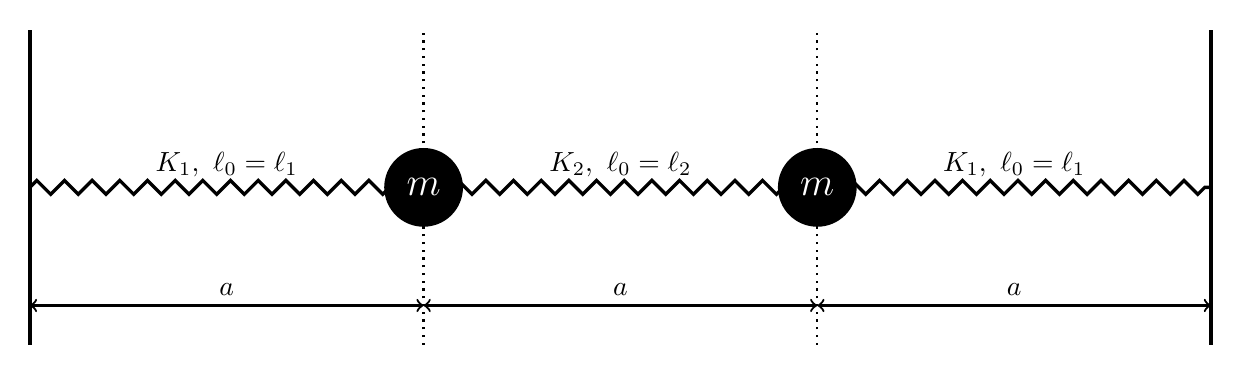
\begin{tikzpicture}

\coordinate (A) at (-2.5,0);
\coordinate (B) at (2.5,0);

\draw[ultra thick](-7.5,-2)--(-7.5,2);
\draw[ultra thick](7.5,-2)--(7.5,2);

\draw[dotted,thick](-2.5,-2)--(-2.5,2);
\draw[dotted,thick](2.5,-2)--(2.5,2);

\draw[<->,thick](-7.5,-1.5)--node[anchor=south]{$a$}(-2.5,-1.5);
\draw[<->,thick](-2.5,-1.5)--node[anchor=south]{$a$}(2.5,-1.5);
\draw[<->,thick](2.5,-1.5)--node[anchor=south]{$a$}(7.5,-1.5);

\draw[very thick,snake=zigzag](-7.5,0)--node[anchor=south]{$K_1,\ \ell_0=\ell_1$}(A);
\draw[very thick,snake=zigzag](A)--node[anchor=south]{$K_2,\ \ell_0=\ell_2$}(B);
\draw[very thick,snake=zigzag](B)--node[anchor=south]{$K_1,\ \ell_0=\ell_1$}(7.5,0);


\fill(A)circle(0.5)node{\color{white} \Large {$m$}};
\fill(B)circle(0.5)node{\color{white} \Large {$m$}};

\end{tikzpicture}
\end{document}